%In data-intensive applications, input data are divided into multiple splits that can be processed in parallel. 

To deal with crash failures, the Shadow Computing computational model can be applied, with one fast replica and one slow replica assigned to process each data partition. While each fast replica runs on one processor exclusively, multiple slow replicas could be collocated to save power and computing resources. A pair of fast and slow replicas for a partition will process the partition from two opposite ends, and complete the task by meeting in an rendezvous point. If one replica fails, however, its associated replica can continue and process the remaining data, potentially with a higher execution rate to minimize delay. Assuming at most 1 failure, the execution dynamics are depicted in Figure~\ref{fig:crash_failure_model}. %The case where both replicas fail simultaneously is ignored due to its extremely low probability. 

\begin{figure}[!t]
	\begin{center}
		\subfigure[Non-faulty task.]
		{
			\label{fig:crash1}
			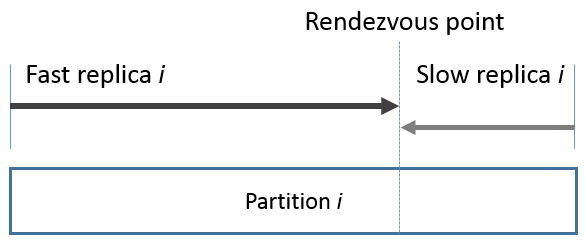
\includegraphics[width=0.9\columnwidth]{figures/crash1}
		}
		\subfigure[Fast replica failure.]
		{
			\label{fig:crash2}
			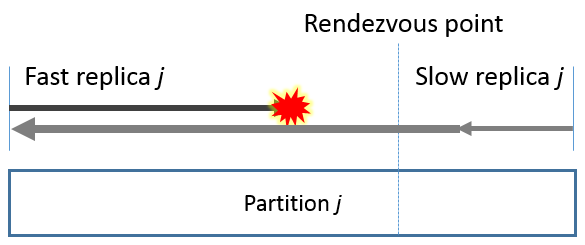
\includegraphics[width=0.9\columnwidth]{figures/crash2}
		}
        \subfigure[Slow replica failure.]
		{
			\label{fig:crash3}
			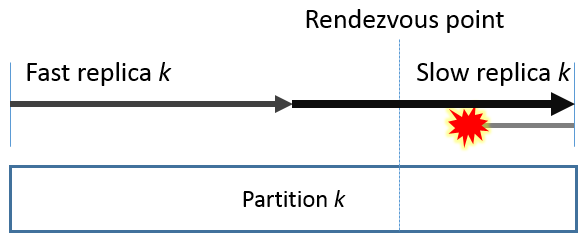
\includegraphics[width=0.9\columnwidth]{figures/crash3}
		}
	\end{center}
	\caption{Illustration of the three possible scenarios when using a pair of fast and slow replicas to process one data partition.}
	\label{fig:crash_failure_model}
\end{figure}

Note that when multiple slow replicas are collocated, to speed up one slow replica (after its associated replica fails) all the other collocated replicas need be terminated. As a result, the fast replicas associated with the terminated slow replicas also need to continue beyond the rendezvous point to process the whole partition. To facilitate the analysis of such correlation, we define \textit{shadowed set} as a set of fast replicas and their collocated slow replicas. The following subsections develop analytical models for the expected response time and energy consumption, given a failure distribution, and then formulate an optimization framework. 

\subsection{Notations}
Let $W$ denote the total amount of workload to process, and $N$ denote the number of processors available. Let $\sigma_{max}$ denote the maximal execution rate of a processor, then $R_{min}=\frac{W}{N \times \sigma_{max}}$ is the minimal response time when no failure occurs. Let $\overline{R}=(1+\alpha)R_{min}$ denote the target response time considering fault tolerance. Let $\lambda$ denote the processor failure rate, and $f(t)$ denote the failure density function. Let $E(\sigma, [t_1, t_2])$ denote the energy consumption of a processor when executing at rate $\sigma$ for an interval from $t_1$ to $t_2$.

According to the dynamics of the Soft Replication model, each processor may run at one of the following four rates:
\begin{itemize}
	\item $\sigma_{m}^{b}$, the initial rate of a processor running a fast replica
    \item $\sigma_{s}^{b}$, the initial rate of a processor running one or more slow replicas
    \item $\sigma_{m}^{a}$, the rate of a processor running a fast replica after speeding up
    \item $\sigma_{s}^{a}$, the rate of a processor running a slow replica after speeding up
\end{itemize}

\subsection{Process execution rates}
It is not difficult to derive the execution rate of each process. Since fast replicas have exclusive access to processors, their execution rates are equal to the rates of the processors that they execute on, i.e., the rate of a fast replica before/after speeding up is  $\sigma_{m}^{b}$/$\sigma_{m}^{a}$. For slow replicas, however, the execution rate depend on not only processor rate, but also on collocation ratio. Let $m$ and $n$ denote the number of processors allocated for fast and slow replicas, respectively. Collocation ratio is then derived as $m/n$, as there will be $m$ pairs of fast and slow replicas and the $m$ slow replicas will share the $n$ processors. Assuming each slow replica gets a fair share of the collocated processor's execution time, the initial rate of a slow replica is $\frac{n}{m}\sigma_{s}^{b}$. After a fast replica failure, process termination is applied so that only the slow replica associated with the failing fast replica remains. Therefore, its effective execution rate is equal to the processor rate, which is $\sigma_{s}^{a}$. 


\subsection{Response time}
\label{sec:res_time}
With a total workload of $W$ and $m$ pairs of replicas, the workload is split into $m$ ways, so the workload for each data partition is $w = W/m$.
For a shadowed set, there are three possible scenarios to consider based on the occurrence of failure, i.e., none of the processors fails, a single processor executing a fast replica fails, or a single processor executing all the slow replicas fails. The case where more than one processor fail simultaneously is ignored due to the extremely low probability.

If no processor fails, each pair of fast and slow replicas will eventually meet at the rendezvous point, which is determined by their relative execution rates. When they meet, the workload done by the fast replica plus the workload by the slow replica should be equal to $w$, and this can lead to the equation $$\sigma_m^b \times t_r^n + \frac{n}{m}\sigma_s^b \times t_r^n = w,$$ where $t_r^n$ denotes the response time when no failure occurs. Using the above equation, it is not difficult to derive that $t_r^n = \frac{w}{\sigma_m^b+\frac{n}{m}\sigma_s^b}$.

If the processor executing slow replicas fails at time $t_f$ before the rendezvous point, all fast replicas speed up to $\sigma_m^a$ and process all the remaining data in each partition. At the time of the failure, the remaining workload for each fast replica is $(w-\sigma_m^b \times t_f)$. Thus, the response time in this case can be expressed as $t_r^m = t_f + \frac{w-\sigma_m^b \times t_f}{\sigma_m^a}$.

In the last scenario, a processor executing a fast replica fails at some time, let's say $t_f$. The associated slow replica speeds up to $\sigma_s^a$ and processes all the remaining data in the partition.  At the time of the failure, the remaining workload for the slow replica is $(w-\frac{n}{m}\sigma_s^b \times t_f)$. The response time in this case can be expressed as $t_r^s = t_f + \frac{w-\frac{n}{m}\sigma_s^b \times t_f}{\sigma_s^a}$.


\subsection{Power and energy}
\label{sec:power_model}
Dynamic voltage and frequency scaling
(DVFS) is a widely available technique to reduce processor frequency. It
is well known that one can reduce the dynamic processor power consumption at
least quadratically by reducing the frequency linearly. The
dynamic processor power consumption executing at rate
$\sigma$ is given by the function $p_d(\sigma)=\sigma^n$ where $n \ge
2$. Throughout this paper we assume that dynamic power is cubic
in relation to processor frequency.

In addition to the dynamic power, processor leakage and other components
(memory, disk, network etc.) all contribute to static power
consumption, which is independent of the processor frequency. In this paper, we
define static power as a fixed fraction of the total power consumed
when executing at maximum rate, referred to as $\rho$. Hence, a processor'
power consumption is expressed as
$p(\sigma)=\rho \times \sigma_{max}^3 + (1-\rho)\times \sigma^3$. 

Using the above power model, the
energy consumed by a processor executing at rate $\sigma$ during an
interval $(t_2-t_1)$ is given by 
$E(\sigma,[t_1, t_2]) = p(\sigma) \times (t_2-t_1)$. 
Considering a shadowed set as a whole and the failure of a processor as a unit, the energy consumption also falls into three cases. Note that each shadowed set contains $m/n$ pairs of replicas, using $(m/n + 1)$ processors. 

If no failure occurs, the energy consumption of a shadowed set, weighted by its probability, is 
\begin{equation}
\begin{split}
E_1 = & (1-\int_{0}^{t_r^n} f(t)dt)^{\frac{m}{n}+1} \times \\
      & \{\frac{m}{n}E(\sigma_m^b,[0,t_r^n])+E(\sigma_s^b,[0,t_r^n])\}
%E_1 = & (1-\int_{0}^{t_r^n} f_m(t)dt)^{\frac{m}{n}} \times (1-\int_{0}^{t_r^n} f_s(t)dt) \times \\
%      & \{\frac{m}{n}E(\sigma_m^b,[0,t_r^n])+E(\sigma_s^b,[0,t_r^n])\}
\label{eq:energy_no_failure}
\end{split}
\end{equation}
The first line is the probability that none of the $m/n$ fast replica processors fails and the slow replica processor also does not fail. The second line captures the energy of all the processors in a shadowed set during the execution. 

If the slow replica processor fails, all the fast replica processors in the shadowed set will speed up. The weighted energy consumption is 
\begin{equation}
\begin{split}
E_2 = & (1-\int_{0}^{t_r^n} f(t)dt)^\frac{m}{n} \times \\
      & \int_{0}^{t_r^n} \{\frac{m}{n}E(\sigma_m^b, [0,t])+E(\sigma_s^b, [0,t]) \\       & +\frac{m}{n}E(\sigma_m^a, [t,t_r^m])\} \times f(t)dt
%E_2 = & (1-\int_{0}^{t_r^n} f_m(t)dt)^\frac{m}{n} \times \\
%      & \int_{0}^{t_r^n} \{\frac{m}{n}E(\sigma_m^b, [0,t])+E(\sigma_s^b, [0,t]) \\       & +\frac{m}{n}E(\sigma_m^a, [t,t_r^m])\} \times f_s(t)dt
\end{split}
\end{equation}   
The energy contains the part of all the processors before the failure, and that of the fast replica processors executing at a higher rate until the completion. 

If a fast replica processor fails, the slow replica processor and all remaining fast replica processors speed up. The weighted energy consumption is 
\begin{equation}
\begin{split}
E_3 = & \frac{m}{n} \times (1-\int_{0}^{t_r^n} f(t)dt)^{\frac{m}{n}}  \times \\
      & \int_{0}^{t_r^n} \{\frac{m}{n} \times E(\sigma_m^b, [0,t]) + (\frac{m}{n}-1)E(\sigma_m^a,[t, t_r^m]) + \\ 
      & +E(\sigma_s^b, [0,t])+E(\sigma_s^a, [t,t_r^s])\} \times f(t)dt
%E_3 = & \frac{m}{n}(1-\int_{0}^{t_r^n} f_m(t)dt)^{\frac{m}{n}-1} \times (1-\int_{0}^{t_r^n} f_s(t)dt) \times \\
%      & \int_{0}^{t_r^n} \{\frac{m}{n} \times E(\sigma_m^b, [0,t]) + (\frac{m}{n}-1)E(\sigma_m^a,[t, t_r^m]) + \\ 
%      & +E(\sigma_s^b, [0,t])+E(\sigma_s^a, [t,t_r^s])\} \times f_m(t)dt
\end{split}
\end{equation}  
The factor of $\frac{m}{n}$ in the probability reflects the possibility that any of the fast replica processors may fail. In addition to the energy consumed before the failure, the above equation also calculates the energy of the remaining processors after speeding up. 

The total energy consumption of the entire job is the sum of the above three, multiplied by the number of shadowed set, i.e., $E_{total}=n \times (E_1+E_2+E_3)$.

\subsection{Shadowed set vulnerability}
As a side effect of collocation, each shadowed set can only tolerate one crash failure, and a second failure will result in a re-execution.  If a second failure in a shadowed set occurs, this situation is referred to as a \textit{shadowed set failure}. It is not difficult to see that the probability of such case depends on the number of processors in each shadowed set and the failure likelihood of each processor. The following part models the shadowed set failure probability. 

Given the response time calculated in above section, the probability of a processor failure during a job's execution is $\int_{0}^{t_r^n} f(t)dt$. For a shadowed set with $\frac{m}{n}+1$ processors, the probability that no processor fails is $P_0=(1-\int_{0}^{t_r^n} f(t)dt)^{\frac{m}{n}+1}$, and the probability that there is exactly one failure is $P_1 = (\frac{m}{n}+1) \times \int_{0}^{t_r^n} f(t)dt \times (1-\int_{0}^{t_r^n} f(t)dt)^{\frac{m}{n}}$.
Since there need to be at least two failures for a shadowed set to fail. the shadowed set failure probability is $P_{set} = 1 - P_0 - P_1$. 


\subsection{Optimization}
\label{sec:crash_opt}
An optimization problem can be formulated to derive the optimal execution rates for both the fast and slow replicas, as well as the optimal collocation ratio for the slow replicas, given an objective and constraint(s). Below we show a case study that minimizes the total energy consumption while meeting response time constraint. 

\begin{equation}
\begin{alignedat}{2}
\min_{\sigma_m^b,\sigma_s^b,\sigma_m^a,\sigma_s^a, m, n} \qquad  & E_{total}(W,N,\overline{R},\rho,\lambda,\sigma_{max},F_t) \\
s.t.  \qquad          & 0 \leq \sigma_m^b \leq \sigma_{max} \\
                      & 0 \leq \frac{n}{m}\sigma_s^b \leq \sigma_m^b \\
                     & \sigma_m^b \leq \sigma_m^a \leq \sigma_{max} \\
                     & \frac{n}{m}\sigma_s^b \leq \sigma_s^a \leq \sigma_{max} \\
                     & 1 \leq n \leq m \leq N \\
                      & max(t_r^n, t_r^m, t_r^s) \leq \overline{R} \\
                      & P_{set} < F_t
\end{alignedat}
\end{equation}

The first constraint says the initial rate of a fast replica should observe the physical processor limit. The second constraint indicates that the initial rate of a slow replica should not exceed that of a fast replica. The third and fourth constraints ensure that fast and slow replicas could speed up after detecting a failure. The next constraint guarantees that the deadline is met even in the presence of failure. Although $t_r^m$ and $t_r^s$ depend on the failure occurrence time, it is clear that the most demanding condition is that if failure occurs at the last moment before reaching the rendezvous point, the remaining replica can still process the entire partition before the deadline. The last constraint can be applied if there is a desire for a threshold on the probability that the job needs to be re-executed.